\documentclass[xcolor=dvipsnames]{beamer}
\mode<presentation> {

\usecolortheme{default}
%\setbeamercovered{transparent}

\definecolor{carolina}{HTML}{82CAFA}
%\definecolor{carolina}{HTML}{3BB9FF}
%\definecolor{gray}{HTML}{B6B6B4}
%\definecolor{dark}{HTML}{151B54}

\usetheme{Madrid}
\setbeamercolor{structure}{fg=carolina}
\setbeamercolor{block title}{bg=carolina}

%Uncomment the following if you prefer for the font color on carolina blue background to be black.
%\setbeamercolor{block title}{fg=black,bg=carolina}
%\setbeamercolor{frametitle}{fg=black}
%\setbeamercolor{title}{fg=black}

\setbeamertemplate{caption}[numbered]
\setbeamertemplate{enumerate items}[circle]
\setbeamertemplate{itemize items}[circle]
\setbeamertemplate{section in toc}[circle]
\setcounter{tocdepth}{1} 
\setbeamercolor{section in toc}{fg=black}

\usefonttheme[onlymath]{serif}

%\setbeamertemplate{footline} % To remove the footer line in all slides uncomment this line
%\setbeamertemplate{footline}[page number] 

% To replace the footer line in all slides with a simple slide count uncomment this line
%\setbeamertemplate{navigation symbols}{}

% To remove the navigation symbols from the bottom of all slides uncomment this line
}

%some commonly used packages
\usepackage{graphics}
\usepackage{graphicx}
\usepackage{tikz}
\usepackage{fancyvrb}
\usepackage[maxbibnames=5, style=nature]{biblatex}
\usepackage{comment}
\usepackage{amsmath}
\usepackage{amssymb}
\usepackage{lipsum}
\usepackage{caption}
\usepackage{comment}
\usepackage{multi row}
\usepackage{mdwlist}

\newcommand{\overbar}[1]{\mkern 1.5mu\overline{\mkern-1.5mu#1\mkern-1.5mu}\mkern 1.5mu} %Instead of \bar or \overline, use \overbar for proper length and thickness bar for sample average. 

%Edit the following lump of code to customize with your name, title, and date
\title[lodr]{Regression with Biomarkers Subject to Lower Limits of Detection}
\author[Donovan, Hudgens, Psioda, and Loop]{Kevin Donovan}
\institute[UNC]{University of North Carolina at Chapel Hill}
\date[8/6/2020]{8/6/2020}

\newcounter{saveenumi}
\newcommand{\seti}{\setcounter{saveenumi}{\value{enumi}}}
\newcommand{\conti}{\setcounter{enumi}{\value{saveenumi}}}
\newcounter{tempcounter}

\resetcounteronoverlays{saveenumi}
\setbeamertemplate{bibliography item}{\insertbiblabel}

\addbibresource{JSM_2020.bib}

\begin{document}

\begin{frame}
	\titlepage
	\begin{figure}
%		\begin{center}
%			\includegraphics[scale = 0.5]{logo_blueonwhite_small.jpg}
%		\end{center}
	\end{figure}
\end{frame}

%\begin{frame}
	%\frametitle{Overview}
	%\setcounter{tocdepth}{2}
	%\tableofcontents
%\end{frame}

\section{Motivation}
\begin{frame}
\frametitle{\insertsectionhead}
\textbf{Adolescent Medicine Trials Network for HIV/AIDS Interventions (ATN) }
\begin{itemize}
\item Study: ATN 071
\item Objective: Analyze associations between selected biomarkers and various neurocognitive outcomes in Youth with HIV
\item Challenge: Measurement error for many biomarkers due to lower limits of detection (LOD) (ex. viral load: 50 copies/mL)
\end{itemize}
\begin{figure}
	\begin{center}
		
\includegraphics[scale = 0.2]{atn_logo.png}
	\end{center}
\end{figure}

\end{frame}

\begin{frame}
\frametitle{\insertsectionhead}
\textbf{Study sample}
\begin{itemize}
\item 128 Youth with HIV
\item Neurocognitive outcomes: \\
Motor, Attention, Executive Functioning, Verbal Nonmemory, Visuospatial Memory (composite Z scores)
\item Composites = means of test performance Z scores
\item Biomarkers: grouped by biological association
	\begin{enumerate}
	\item Macrophage Activation (10 biomarkers, 3 with LOD)
	\item Vascular Inflammation (4 biomarkers, 0 with LOD)
	\item Lymphocyte Activation (4 biomarkers, 3 with LOD)
	\end{enumerate}
\end{itemize}
\end{frame}

\begin{frame}
\frametitle{\insertsectionhead}
\textbf{Analytic Strategy}
\begin{itemize}
\item Proportion of sample values under LOD:
\begin{enumerate}
\item GM-CSF: 41\%\  (LOD = 0.01 pg/mL)
\item IL-1$\beta$: 26\%\ (LOD = 0.01 pg/mL)
\item IL-6: 20\%\ (LOD = 0.1 pg/mL)
\item INF$\gamma$: 38\%\ (LOD = 0.1 pg/mL)
\item IL-10: 27\%\ (LOD = 0.1 pg/mL)
\item sIL-2r$\alpha$: 1\%\ (LOD = 0.1 pg/mL)
\item Viral Load: 62\%\ (LOD = 50 copies/mL)
\end{enumerate}
\item Fit linear regression models for each pair of neurcognitive domain scores and biomarker group (15 total models)
\begin{itemize}
\item Outcome = neurocognitive domain scores;\\
Covariates = biomarkers in group and potential confounders (ex. viral load, gender, race) 
\end{itemize}
\end{itemize}
\end{frame}

\section{Methodology}
\begin{frame}
\frametitle{\insertsectionhead}
\textbf{In literature}
\begin{itemize}
\item Substitution: use LOD/function of LOD value ($/\sqrt{2}$) \cite{nie_2012}
\item Maximum likelihood (ML) with observed only:\\
likelihood generally derived with very limited number of covariates  \cite{lynn_2001, cole_2009, nie_2012}
\item Bayesian estimation \cite{wu_2012}
\item \textbf{ML using Expectation-Maximization (EM)}: allows for arbitrary number of LOD/non-LOD covariates \cite{may_2011}
\end{itemize}
\end{frame}

\begin{frame}
\frametitle{\insertsectionhead}
\textbf{May et al. 2011}\\
\vspace{0.5cm}
Model Overview:\\
Assume random sample of $n$ independent observations of\\
$(Y_i, X_i)$ for $i=1,\ldots,n$\\
$X_i$ is a set of $p$ covariates with $X_i \sim N_p(\mu_X, \Sigma_X)$,\\
$Y_i|X_i \sim N(\mu_i, \sigma^2)$ and $\mu_i=\beta_0+\beta_1X_{i,1}+\ldots+\beta_pX_{i,p}$ for $i=1,\ldots,n$\\ 
\vspace{0.5cm}
For simplicity, assume covariates $X_{i,q}, X_{i,q+1}, \ldots, X_{i,p}$\\
are subject to LODs for $0<q \leq p$
\end{frame}

\begin{frame}
Let $Y=(Y_1, \ldots, Y_n)$ and $X$ be the $n$ by $p$ martix of covariates.\\
If all covariates were fully observed (all inside LODs), the conditional log likelihood function would be\\
$$L(\theta | Y, X) = \sum_{i=1}^n \textrm{log}[f(Y_i | X_i, \theta)],$$\\ where $\theta = (\beta, \sigma^2)$ and $\beta=(\beta_0, \dots, \beta_p)$\\
\vspace{0.5cm}
Covariates with LODs may be unobserved $\implies$ model joint log likelihood instead:\\
$$L(\gamma | Y, X) = \sum_{i=1}^n \textrm{log}[f(Y_i | X_i, \theta) f(X_i | \alpha)]$$ where $\gamma=(\theta, \alpha)$, $\alpha=(\mu_X, \Sigma_X)$, $X_i=(X_{i,1} \ldots,$ and $X_{i,p})$
\end{frame}

\begin{frame}
LODs $\implies$ $X_i$ can be partitioned into $X_i=(X_{i,obs}, X_{i,cens})$\\
where $X_{i,obs}$ denotes covariates with fully observed values,\\
$X_{i,obs}$ denotes covariates with values outside of their LODs\\
\vspace{0.5cm}
To maximize $L(\gamma | Y, X)$ with respect to $\gamma$, use E-M algorithm due to missing covariate values.\\
\vspace{0.5cm}
Let $\hat{\gamma}^{(t)}$ denote the estimate of $\gamma$ at iteration $t$.\\
For simplicity, suppose $i=m, m+1, \dots, n$ where $0<m \le n$ have covariate values outside of LODs. 
\end{frame}

\begin{frame}
Let $Y=(Y_1, \ldots, Y_n)$ and $X$ be the $n$ by $p$ martix of covariates.\\
If all covariates were fully observed (all inside LODs), the conditional log likelihood function would be\\
$$L(\theta | Y, X) = \sum_{i=1}^n \textrm{log}[f(Y_i | X_i, \theta)],$$\\ where $\theta = (\beta, \sigma^2)$ and $\beta=(\beta_0, \dots, \beta_p)$\\
\vspace{0.5cm}
Covariates with LODs may be unobserved $\implies$ model joint log likelihood instead:\\
$$L(\gamma | Y, X) = \sum_{i=1}^n \textrm{log}[f(Y_i | X_i, \theta) f(X_i | \alpha)]$$ where $\gamma=(\theta, \alpha)$, $\alpha=(\mu_X, \Sigma_X)$, $X_i=(X_{i,1} \ldots,$ and $X_{i,p})$
\end{frame}

\begin{frame}
\textbf{E-M Algorithm}\\
Expectation (E) step:
\begin{align*}
Q(\gamma | \hat{\gamma}^{(t)})&=\textrm{E}[L(\gamma | Y, X)|Y, X_{obs}] \\
 &= \sum_{i=1}^{m-1}\textrm{log}[f(Y_i | X_i, \theta) f(X_i | \alpha)] \\
 &+ \sum_{i=m}^n\textrm{E}(\textrm{log}[f(Y_i | X_i, \theta) f(X_i | \alpha)]|Y_i,X_{i, \textrm{obs}})
\end{align*}
where $X_{obs}$ denotes the observed covariate values for all $n$ observations.\\
\vspace{0.5cm}
$\textrm{E}(\textrm{log}[f(Y_i | X_i, \theta) f(X_i | \alpha)]|Y_i,X_{i, \textrm{obs}})$ often does not have a closed form \cite{may_2011}\\
$\implies$\\
Monte Carlo approximation is used for this term for $m \leq i \leq n$.
\end{frame}

\begin{frame}
\textbf{Monte Carlo Approximation}\\
Suppose $Z$ has density function $f(z)$.\\
Given $Z_1, \ldots, Z_n$ i.i.d from $f(z)$ for $n>0$,\\
the Monte Carlo approximation of $E(Z)$ is $\sum_{i=1}^n Z_i/n$\\
\vspace{0.5cm}
Thus in the E step above, define Monte Carlo approximation
$$\hat{\textrm{E}}(\textrm{log}[f(Y_i | X_i, \theta) f(X_i | \alpha)]|Y_i,X_{i, \textrm{obs}})=\sum_{j=1}^{r_i} \textrm{log}[f(Y_i | Z_i, \theta) f(Z_i | \alpha)]/r_i$$\\ for $i=m, \ldots, n$ where $Z_{i,j}$ i.i.d from truncated distribution of $X_{i,cens}|X_{i,obs},Y_i,c_l<X_{i,cens}<c_u$\\
\vspace{0.5cm}
The corresponding approximated E step is
\begin{align*}
\hat{Q}(\gamma | \hat{\gamma}^{(t)})&=\sum_{i=1}^{m-1}\textrm{log}[f(Y_i | X_i, \theta) f(X_i | \alpha)]\\
 &+ \sum_{i=m}^n\hat{\textrm{E}}(\textrm{log}[f(Y_i | X_i, \theta) f(X_i | \alpha)]|Y_i,X_{i, \textrm{obs}})
 \end{align*}
\end{frame}

\begin{frame}
Plugging-in the Monte Carlo expectation and rearranging terms results in
\begin{align*}
\hat{Q}(\gamma | \hat{\gamma}^{(t)})&=\sum_{i=1}^{m-1}\textrm{log}[f(Y_i | X_i, \theta) f(X_i | \alpha)]\\ 
&+\sum_{i=m}^n\sum_{j=1}^{r_i}\textrm{log}[f(Y_i | Z_{i,j}, \theta) f(Z_{i,j} | \alpha)]/r_i\\
&= \sum_{i=1}^{m-1}\textrm{log}[f(Y_i | X_i, \theta)]+
\sum_{i=m}^n\sum_{j=1}^{r_i}\textrm{log}[f(Y_i | Z_{i,j}, \theta)]/r_i\\
&+ \sum_{i=1}^{m-1}\textrm{log}[f(X_i | \alpha)]+
\sum_{i=m}^n\sum_{j=1}^{r_i}\textrm{log}[f(Z_{i,j} | \alpha)]/r_i
\end{align*}

thus the maximization step can be applied to obtain $\theta$ and $\alpha$ separately.
\end{frame}

\begin{frame}
\textbf{Maximization (M) step:}\\
Above approx. E step $\implies$\\
$\hat{\theta}$ and $\hat{\alpha}$ obtained by weighted maximum likelihood estimation\\
\vspace{0.5cm}
Regression model $\implies$\\
weighted least squares procedure and weighted sample mean/covariance for $\hat{\theta}$ and $\hat{\alpha}$ respectively\\
\vspace{0.5cm}
weight = 1 for subjects with no covariates outside of LODs,\\
= $r_i$ else.\\
\vspace{0.5cm}
Often $r_i=r$ for all $i$ 
\end{frame}

\begin{frame}
\textbf{M step algorithm:}\\
Per May et al. (2011)\\
For simplicity, assume all observations with missing covariate values have values under the LOD for covariates $X_{i,q}, \dots, X_{i,p}$:\\

\begin{enumerate}
  \item provide starting values $\hat{\gamma}^{(0)}$ by fitting the model on only the observed data (i.e., a "complete case" analysis).  Set the starting values for the sampling procedure to be the means of the covariates subject to a LOD in the observed data only.
  \item at step $t$, for observation $i$ with censored covariates $X_{i,\textrm{cens}}$, sample $X_{i,q,\textrm{cens}}$. Denote this sampled value by $Z_{i,q,1}$.
  \item for observation $i$ conditional on $X_{i,\textrm{obs}}$, $Y_i$, and $Z_{i,q,1}$, sample $X_{i,q+1,\textrm{cens}}$.  Denote this sampled value by $Z_{i,q+1,1}$.
  \item repeat step 2 and 3 until you have sampled values for all $X_{i,\textrm{cens}}$, resulting in vector $Z_{i,1}=(Z_{i,q,1},\dots,Z_{i,p,1})$.
  \setcounter{tempcounter}{\value{enumi}}
\end{enumerate}
\end{frame}

\begin{frame}
\begin{enumerate}
  \setcounter{enumi}{\value{tempcounter}}
\item repeat steps 2-4 $R$ times (e.g., 25) until you have $Z_{i,1}, \dots, Z_{i,R}$
  \item repeat steps 2-5 for all observations with censored covariates.  This results in a new dataset, consisting of one observation (row) $(Y_i, X_i)$ for a subject with fully observed covariate data (i.e., none under a LOD) and $R$ observations (rows) $(Y_i, X_{i,obs}, Z_{i,1}), \dots, (Y_i, X_{i,obs}, Z_{i,R})$ for a subject with at least one covariate under a LOD.
  \item compute $\hat{\gamma}^{(t+1)}$ using weighted least squares with the sampled dataset detailed in step 6, with weight $1/R$ for observations with sampled data. 
  \item repeat steps 2-7 until the absolute difference between $\hat{\gamma}_{t-1}$ and $\hat{\gamma}_{t}$ is less than some predetermined threshold $\epsilon$
\end{enumerate}
\end{frame}

\begin{frame}
\textbf{Standard Error Calculation:}\\
\begin{itemize}
\item Analytical calculation: Louis's method for computing the information matrix \cite{louis_1982}
\item Bootstrap standard errors
\end{itemize}

\textbf{Sampling methods:}\\
\begin{itemize}
\item Recall steps 2-6 involve sampling of unobserved biomarker values to compute Monte Carlo approximation
\item Sampling is most computationally/time intensive portion of algorithm
\item Options:
\begin{enumerate}
\item Adaptive Rejection Metropolis Sampling (ARMS) \cite{gilks_1995},\\
used by May et al. (2011)
\item Slice sampling \cite{neal_2003}
\end{enumerate}
\end{itemize}
\end{frame}

\begin{frame}
\textbf{Standard Error Calculation:}\\
\begin{itemize}
\item Analytical calculation: Louis's method for computing the information matrix \cite{louis_1982}
\item Bootstrap standard errors
\end{itemize}

\textbf{Sampling methods:}\\
\begin{itemize}
\item Recall steps 2-6 involve sampling of unobserved biomarker values to compute Monte Carlo approximation
\item Sampling is most computationally/time intensive portion of algorithm
\item Options:
\begin{enumerate}
\item Adaptive Rejection Metropolis Sampling (ARMS) \cite{gilks_1995},\\
used by May et al. (2011)
\item Slice sampling \cite{neal_2003}
\end{enumerate}
\end{itemize}
\end{frame}

\section{lodr Package}
\begin{frame}
\frametitle{\insertsectionhead}
\textbf{Before: no implementation available}\\
\textbf{Now: linear regression implementation with R package \underline{lodr}}\\
\vspace{0.5cm}
Computationally intensive sampling $\implies$ C++ used for sampling, M step, and bootstrap\\
\begin{figure}
	\begin{center}
		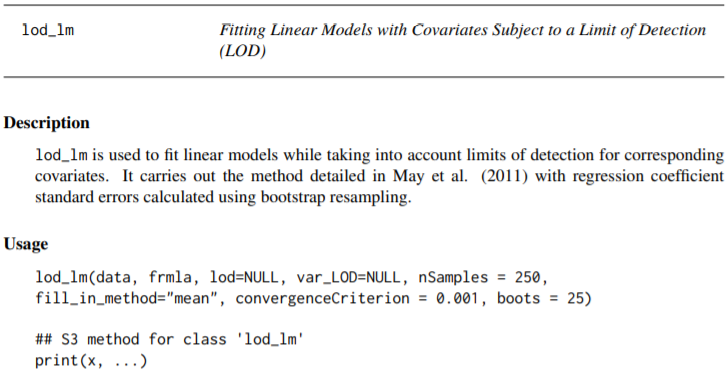
\includegraphics[scale = 0.65]{lod_lm.png}
	\end{center}
\end{figure}
\end{frame}

\begin{frame}
\frametitle{\insertsectionhead}
\textbf{Package mimics lm function in R}\\
Supporting functions:
\begin{itemize}
\item lod\textunderscore lm
\item summary.lod\textunderscore lm
\item coef.lod\textunderscore lm
\item residuals.lod\textunderscore lm
\end{itemize}
\end{frame}

\begin{frame}
\frametitle{\insertsectionhead}
\textbf{Simulation Example}\\
$n=100$; outcome variable $Y$ with 3 covariates ($X_1$, $X_2$, $X_3$)\\
$X_2$ and $X_3$ subject to lower LODs of 0\\
All covariates generated from $N(0,1)$\\
\vspace{0.5cm}
$Y=\beta_0+\beta_1X_1+\beta_2X_2+\beta_3X_3+\epsilon$ where $\beta_0=\ldots=\beta_3=1$
\end{frame}

\begin{frame}
\textbf{Simulation Results:}\\
100 repetitions\\
\begin{figure}
	\begin{center}
		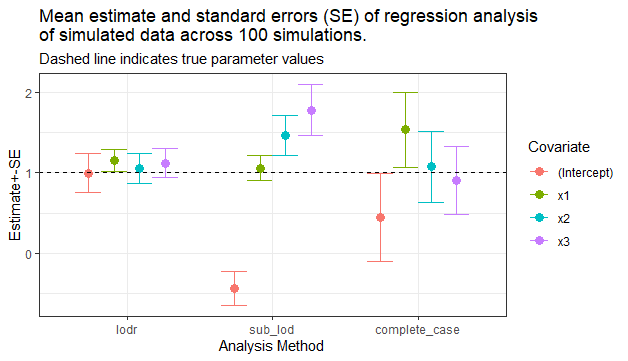
\includegraphics[scale = 0.75]{sim_results.png}
	\end{center}
\end{figure}
\end{frame}

\begin{frame}
\begin{table}[ht]
\centering
\scalebox{0.9}{
\begin{tabular}{llllll}
  \hline
Method & Covariate & Mean Est. & Est. Bias & Mean SE & Mean DF \\ 
  \hline
lodr & (Intercept) & 1.00 & -0.00 & 0.24 & 96.00 \\ 
  lodr & x1 & 1.15 & 0.15 & 0.13 & 96.00 \\ 
  lodr & x2 & 1.05 & 0.05 & 0.19 & 96.00 \\ 
  lodr & x3 & 1.12 & 0.12 & 0.18 & 96.00 \\ 
  \hline
  sub\_lod & (Intercept) & -0.44 & -1.44 & 0.21 & 96.00 \\ 
  sub\_lod & x1 & 1.06 & 0.06 & 0.16 & 96.00 \\ 
  sub\_lod & x2 & 1.47 & 0.47 & 0.25 & 96.00 \\ 
  sub\_lod & x3 & 1.78 & 0.78 & 0.32 & 96.00 \\ 
  \hline
  complete\_case & (Intercept) & 0.44 & -0.56 & 0.55 & 21.30 \\ 
  complete\_case & x1 & 1.54 & 0.54 & 0.47 & 21.30 \\ 
  complete\_case & x2 & 1.08 & 0.07 & 0.44 & 21.30 \\ 
  complete\_case & x3 & 0.91 & -0.09 & 0.42 & 21.30 \\ 
   \hline
\end{tabular}
}
\end{table}
\end{frame}

\section{ATN 071 Analysis}
\begin{frame}
\frametitle{\insertsectionhead}
\textbf{Recall}: regression models run with neurocognitive composite as outcome, group biomarkers as covariates\\
\vspace{0.5cm}
\textbf{Potential confounders}: Age, gender, race, education, employment, income, recent substance use, depression symptoms, and concurrent infections
\end{frame}

\begin{frame}
\frametitle{\insertsectionhead}
\begin{figure}
	\begin{center}
		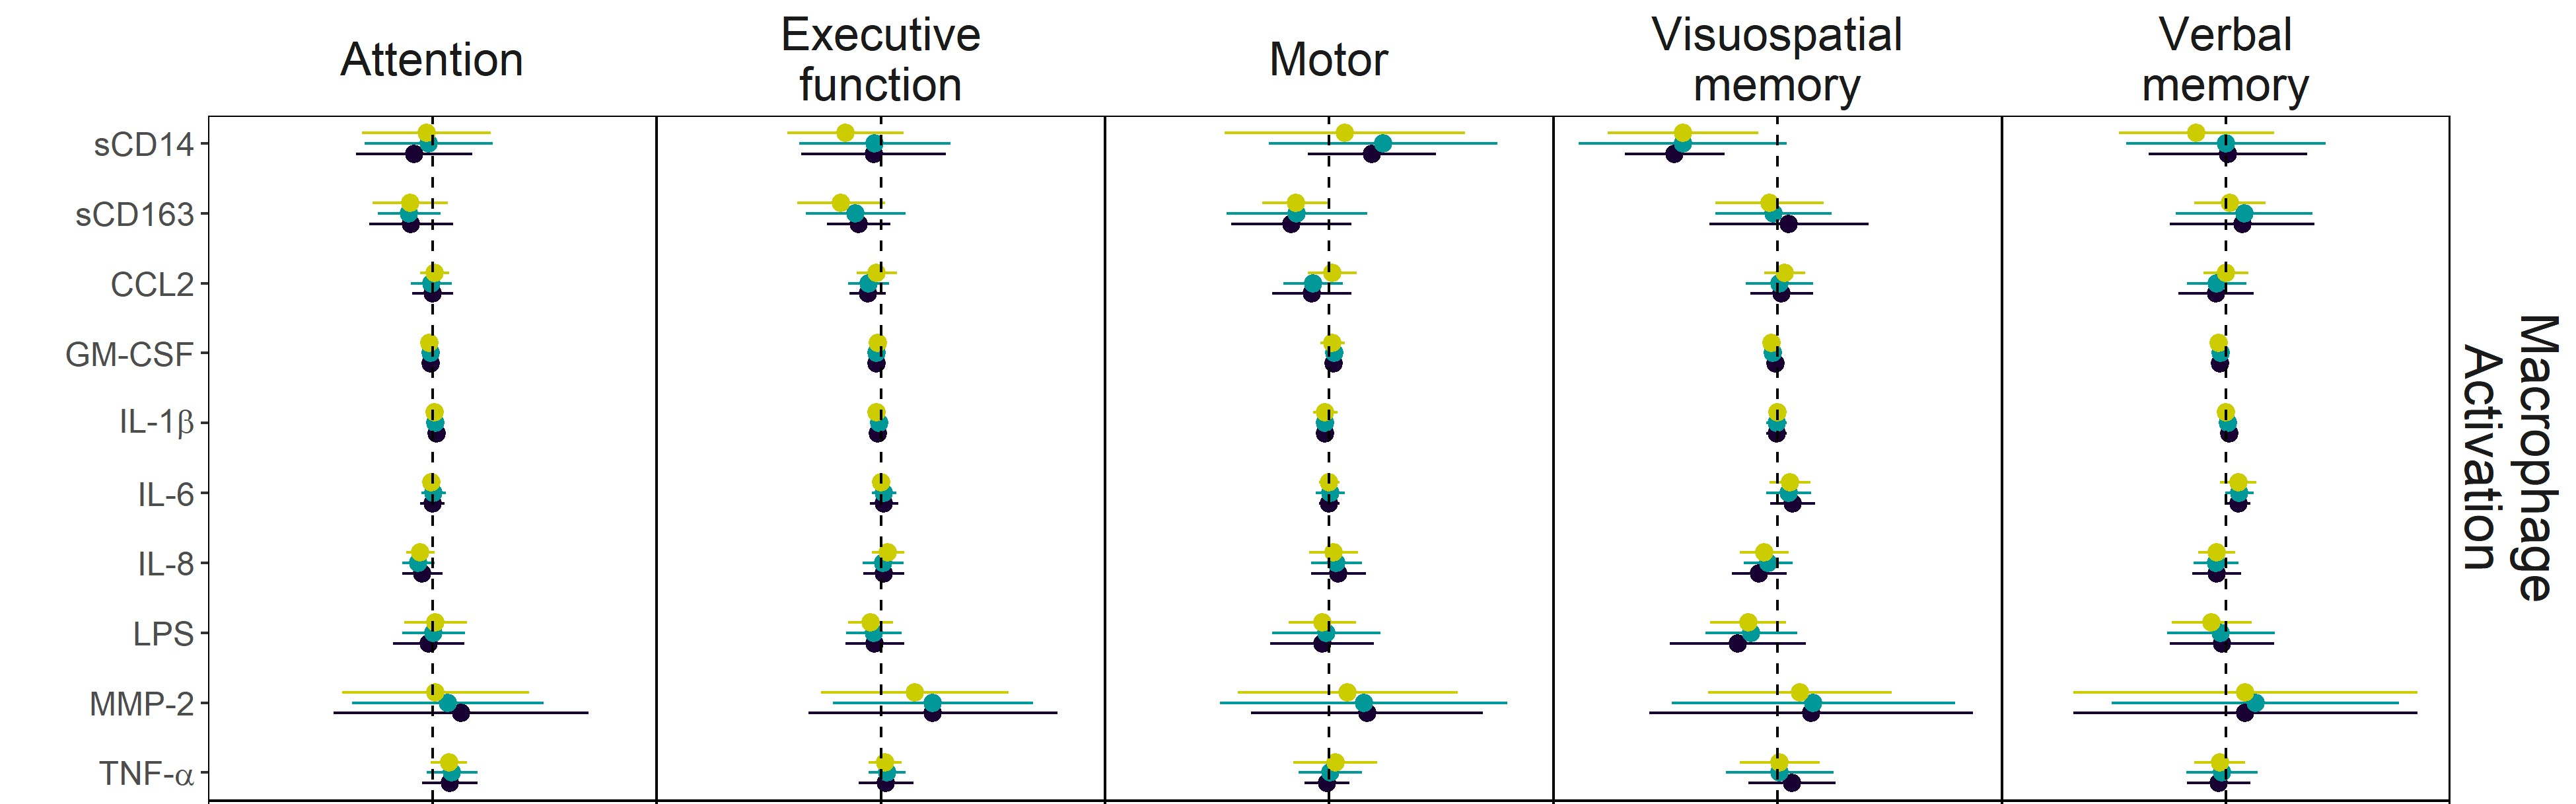
\includegraphics[scale = 0.37]{figure_2_AIDS_top.jpg}
	\end{center}
\end{figure}
\end{frame}

\begin{frame}
\frametitle{\insertsectionhead}
\begin{figure}
	\begin{center}
		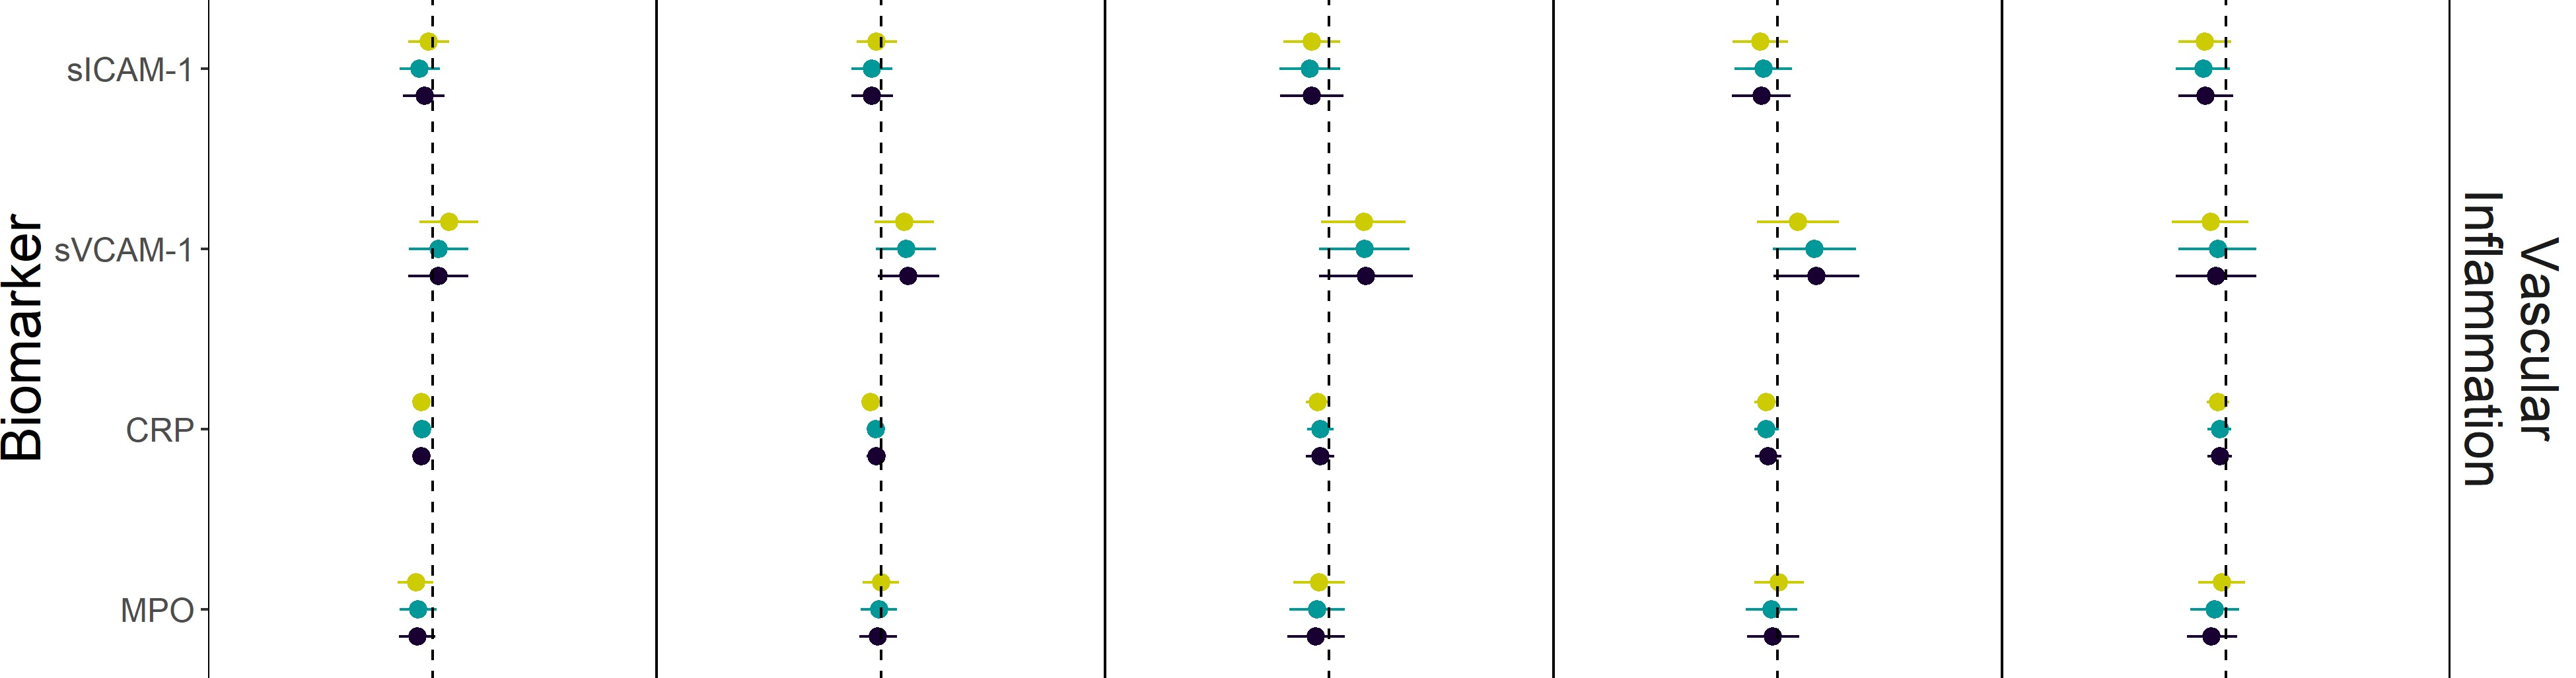
\includegraphics[scale = 0.37]{figure_2_AIDS_middle.jpg}
	\end{center}
\end{figure}
\end{frame}

\begin{frame}
\frametitle{\insertsectionhead}
\begin{figure}
	\begin{center}
		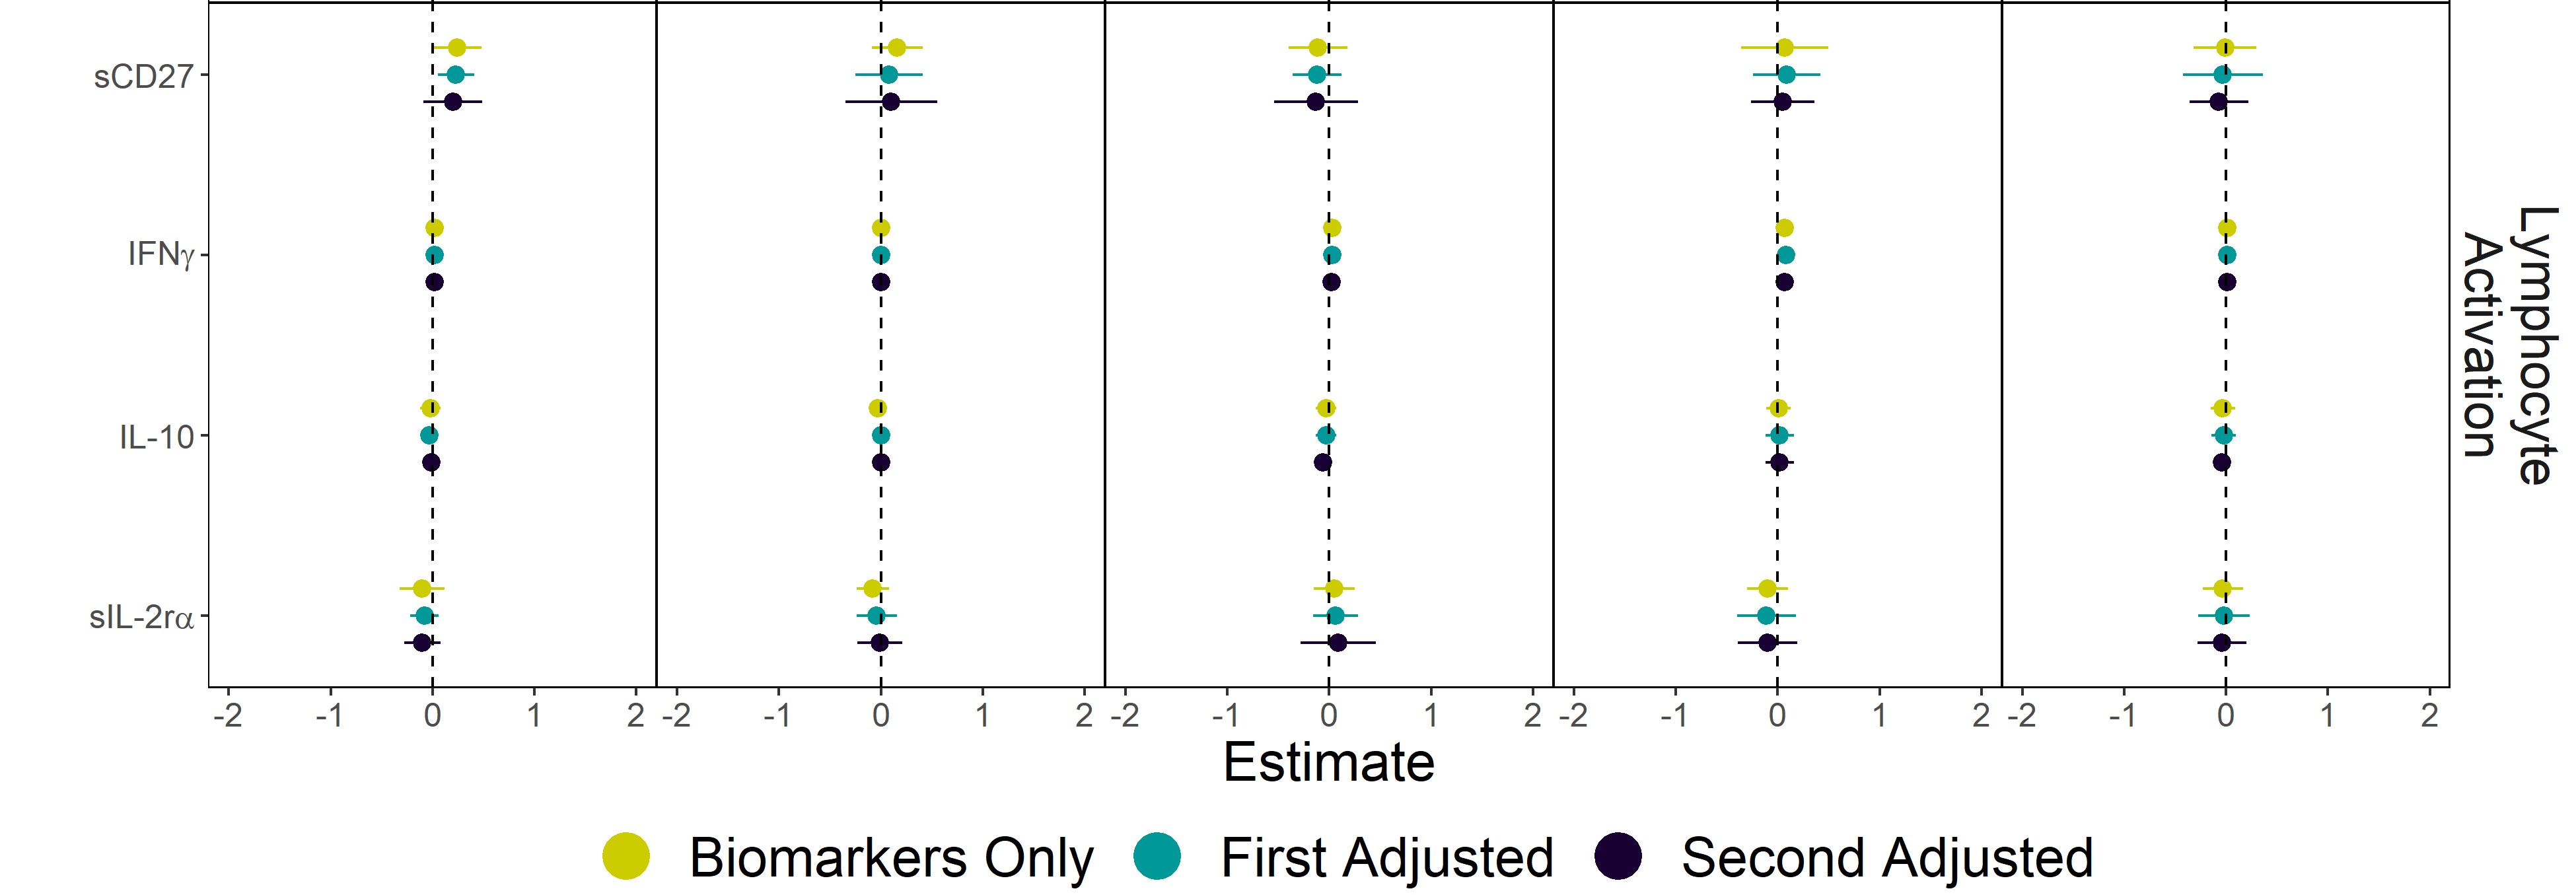
\includegraphics[scale = 0.37]{figure_2_AIDS_bottom.jpg}
	\end{center}
\end{figure}
\end{frame}

\section{Limitations and Future Research}
\begin{frame}
\frametitle{\insertsectionhead}
\begin{itemize}
\item Method requires joint distribution of covariates specified $\implies$
handling categorical covariates difficult \textbf{(ad hoc method applied)}
\item Computational time for large datasets and simulation studies
\item Implementation for generalized linear models in package 
\item Hypothesis testing and handling residuals
\end{itemize}
\end{frame}

\section{Bibliography}
\begin{frame}[allowframebreaks]
\frametitle{\insertsectionhead}
\printbibliography
\end{frame}

\end{document}
